% arara: pdflatex

\documentclass[
    tikz,%
    border={0mm 0mm 0mm 0mm},% left bottom right top
]{standalone}
\usepackage{pgfplots}
\usepackage{amsmath}
\usepackage{siunitx}

\usepgfplotslibrary{units}

\definecolor{seq1}{RGB}{123,204,196}
\definecolor{seq2}{RGB}{67,162,202}
\definecolor{seq3}{RGB}{8,104,172}

\definecolor{seqa}{RGB}{253,204,138}
\definecolor{seqb}{RGB}{252,141,89}
\definecolor{seqc}{RGB}{215,48,31}

\definecolor{seqA}{RGB}{194,230,153}
\definecolor{seqB}{RGB}{120,198,121}
\definecolor{seqC}{RGB}{35,132,67}

\newcommand{\etal}{\mbox{\emph{et al.\ }}}

\begin{document}
\begin{tikzpicture}
% Nature settings:
% For guidance, Nature’s standard figure sizes are 89 mm (single column) and
    % 183 mm (double column) and the full depth of the page is 247 mm.
% Draw exact dimensions bounding box
\newcommand{\figwidth}{8.64cm}
\newcommand{\figheight}{6.915cm} % golden ratio
%\newcommand{\figheight}{6.00cm} % golden ratio
\draw[use as bounding box, white] (0,0) rectangle (\figwidth,\figheight);

 \begin{semilogxaxis}[
    xshift=1.24cm,
    yshift=0.71cm,
    clip mode=individual,
    xmin=2, xmax=400,
    ymin=0.0, ymax=0.15,
    enlargelimits=false,
    axis on top=true,
    xlabel=$d$,
    ylabel=$\text{Probability}$,
    x unit=\si{\micro\metre},
    %y unit=\si{\per\micro\metre},
    legend pos=south west,
    legend style={draw=none, 
                  font=\footnotesize,
                  fill=none,
                 },
    legend cell align=left,
    %legend style={at={(-0.01, 0)}, anchor=south west},
    width = 8.95cm,
    height = 4.5cm,
    ylabel near ticks, 
    xlabel near ticks, 
    %xtick pos=left,
    minor tick num=1,
    %ytick = {0.8, 0.9, 1.0, 1.1, 1.2},
    x label style={yshift=3mm},
    y label style={yshift=-1mm},
    y tick label style={
        /pgf/number format/.cd,
        fixed,
        fixed zerofill,
        precision=2,
        /tikz/.cd
    }
  ]
  \addplot+[
        forget plot,
        mark=none,
        line width=2pt,
        line join=round,
        color=seqB,
    ] table [
        x = bins,
        y = hist,
        col sep=comma,
    ] {dropletdiameters_waterInOil.csv};

    \fill[color=seqA, line join=round] 
    (axis cs: 42.90095139876563,0.0) --
    (axis cs: 42.90095139876563,0.003992015968063872) --
    (axis cs: 49.12363014719691,0.012974051896207584) --
    (axis cs: 56.24889332659474,0.033932135728542916) --
    (axis cs: 64.40765861533495,0.0748502994011976) --
    (axis cs: 73.74983298290371,0.08882235528942116) --
    (axis cs: 84.44706704042804,0.10379241516966067) --
    (axis cs: 96.6959089030573,0.10778443113772455) --
    (axis cs: 110.72141551241927,0.08383233532934131) --
    (axis cs: 126.78128777262246,0.08882235528942116) --
    (axis cs: 145.17060547768727,0.09880239520958084) --
    (axis cs: 166.2272490286948,0.09481037924151696) --
    (axis cs: 190.33810755783273,0.06986027944111776) --
    (axis cs: 217.9461875257477,0.05888223552894212) --
    (axis cs: 249.5587524036703,0.03493013972055888) --
    (axis cs: 285.75664299665203,0.02594810379241517) --
    (axis cs: 327.20494965703773,0.010978043912175649) --
    (axis cs: 374.66523247656886,0.000998003992015968) --
    (axis cs: 374.66523247656886,0.0) -- cycle;

  \addplot+[
        forget plot,
        mark=none,
        line width=2pt,
        line join=round,
        color=seqb,
    ] table [
        x = bins,
        y = hist,
        col sep=comma,
    ] {dropletdiameters_oilInWater.csv};
    
    \fill[color=seqa, line join=round] 
    (axis cs: 2.556630894923492,0.0) --
    (axis cs: 2.556630894923492,0.0025252525252525255) --
    (axis cs: 3.006229984121015,0.015151515151515152) --
    (axis cs: 3.5348938070697473,0.03535353535353535) --
    (axis cs: 4.1565263779755615,0.05176767676767677) --
    (axis cs: 4.887476816489767,0.08712121212121213) --
    (axis cs: 5.746969334369853,0.10858585858585859) --
    (axis cs: 6.75760883790918,0.11363636363636363) --
    (axis cs: 7.94597544362839,0.11363636363636363) --
    (axis cs: 9.343323543166283,0.11616161616161616) --
    (axis cs: 10.986403802982608,0.09595959595959595) --
    (axis cs: 12.918429717706992,0.0946969696969697) --
    (axis cs: 15.1902141377717,0.056818181818181816) --
    (axis cs: 17.861505662339574,0.045454545454545456) --
    (axis cs: 21.00256004505468,0.02904040404040404) --
    (axis cs: 24.695987941049594,0.012626262626262626) --
    (axis cs: 29.03892759149967,0.008838383838383838) --
    (axis cs: 34.14559958796781,0.006313131313131313) --
    (axis cs: 40.1503109075942,0.0025252525252525255) --
    (axis cs: 47.21098722614113,0.0012626262626262627) --
    (axis cs: 55.51332640976588,0.0) -- cycle;

    %\draw[seqb, densely dashed, line width=0.2mm, opacity=1.0]
    %(axis cs: 8.82393067556, 0) -- (axis cs: 8.82393067556, 0.116);
    \draw[seq3, fill=seq2] (axis cs: 8.82393067556, 0.116)
    node[above, black] {\SI{8.8}{\micro\metre}} circle (1pt);

    %\draw[seqB, densely dashed, line width=0.2mm, opacity=1.0]
    %(axis cs: 123.967936904, 0) -- (axis cs: 123.967936904, 0.089);
    \draw[seq3, fill=seq2] (axis cs: 123.967936904, 0.089)
    node[above=5mm, right=-3mm, black] {\SI{124}{\micro\metre}} circle (1pt);
    
    \node[text width=10mm, align=center] at (axis cs: 8.3, 0.045)
    {Oil in water};
    \node[text width=10mm, align=center] at (axis cs: 118, 0.045)
    {Water in oil};

% \node[black] at (1.15cm, 2.70cm) {\textbf{C}};

 \end{semilogxaxis}

 \begin{scope}[
    xshift=0cm,
    yshift=3.9cm,
]
    
% trim: left bottom right top
\node[inner sep=0pt, anchor=south west] (image) at (0,0)
{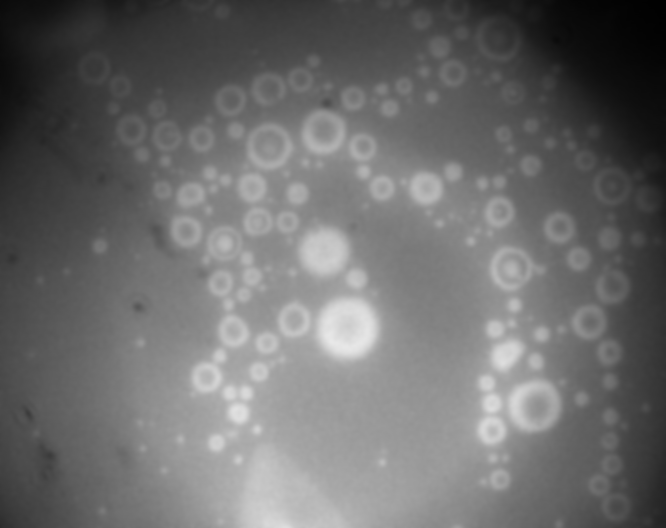
\includegraphics[width=4.3cm,height=3.0cm,clip,
                  trim={0.0cm, 1cm, 0.0cm, 0cm}, 
]{small1.png}};

\node[inner sep=0pt, anchor=south east] (image) at (\figwidth,0)
{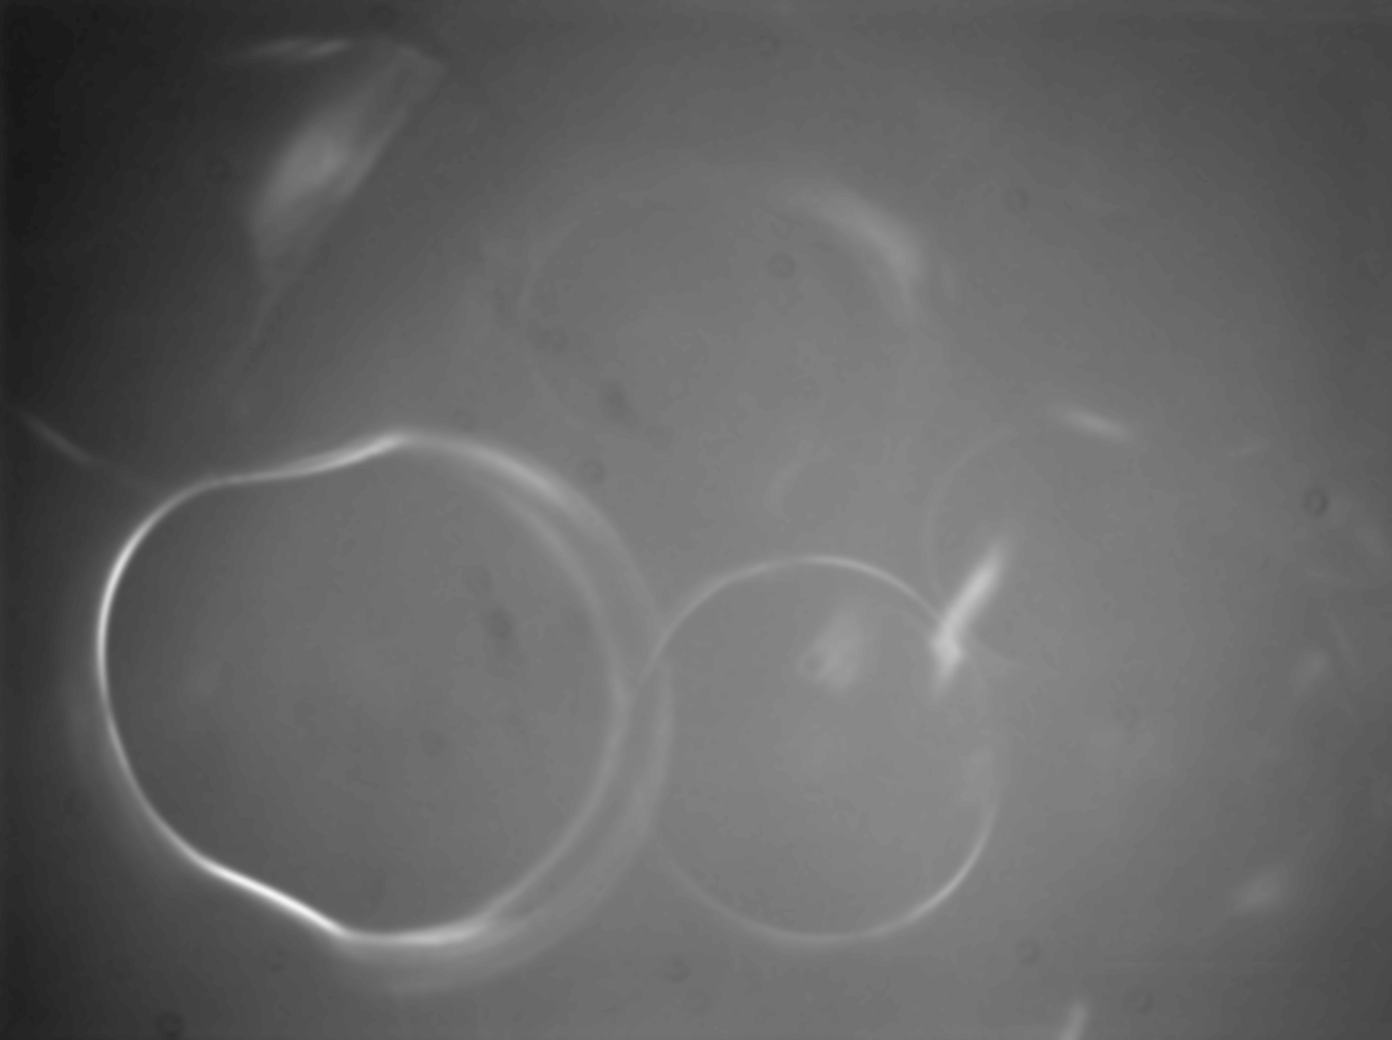
\includegraphics[width=4.3cm,height=3.0cm, clip,
                  trim={0.0cm, 1cm, 0.0cm, 0cm}, 
]{waterinoil2.png}};

% scale bar right
\begin{scope}[
    xshift=7.37cm,
    yshift=2.35cm,
]
   \fill[fill=white, fill opacity=0.25] (0.0mm, 0.0mm) rectangle ++(12mm, 6.0mm);
   \draw [white, line width=0.3em] (1.25mm, 4.7mm) --
       node[below=0.3mm,inner sep=0.1em, font=\normalsize] {\SI{100}{\micro\metre}}
       ++(9.57mm, 0mm);
\end{scope}

% scale bar left
\begin{scope}[
    xshift=3.05cm,
    yshift=2.35cm,
]
   \fill[fill=white, fill opacity=0.25] (0.0mm, 0.0mm) rectangle ++(12mm, 6.0mm);
   \draw [white, line width=0.3em] (5.4mm, 4.7mm) --
       node[below=0.3mm,inner sep=0.1em, font=\normalsize] {\SI{10}{\micro\metre}}
       ++(2.02mm, 0mm);
\end{scope}

% labels
% \node[white] at (0.22cm, 2.80cm) {\textbf{A}};
% \node[white] at (4.55cm, 2.80cm) {\textbf{B}};
\end{scope}

\end{tikzpicture} 
\end{document}
